%  LaTeX support: latex@mdpi.com 
%  For support, please attach all files needed for compiling as well as the log file, and specify your operating system, LaTeX version, and LaTeX editor.

%=================================================================
\documentclass[journal,article,submit,pdftex,moreauthors]{Definitions/mdpi} 
\usepackage{pgf-pie}
\usepackage[justification=centering]{caption}
\usepackage{graphicx} % Untuk gambar
\usepackage{float} % Untuk kontrol posisi gambar

%--------------------
% Class Options:
%--------------------
%----------
% journal
%----------
% Choose between the following MDPI journals:
% acoustics, actuators, addictions, admsci, adolescents, aerobiology, aerospace, agriculture, agriengineering, agrochemicals, agronomy, ai, air, algorithms, allergies, alloys, analytica, analytics, anatomia, animals, antibiotics, antibodies, antioxidants, applbiosci, appliedchem, appliedmath, applmech, applmicrobiol, applnano, applsci, aquacj, architecture, arm, arthropoda, arts, asc, asi, astronomy, atmosphere, atoms, audiolres, automation, axioms, bacteria, batteries, bdcc, behavsci, beverages, biochem, bioengineering, biologics, biology, biomass, biomechanics, biomed, biomedicines, biomedinformatics, biomimetics, biomolecules, biophysica, biosensors, biotech, birds, bloods, blsf, brainsci, breath, buildings, businesses, cancers, carbon, cardiogenetics, catalysts, cells, ceramics, challenges, chemengineering, chemistry, chemosensors, chemproc, children, chips, cimb, civileng, cleantechnol, climate, clinpract, clockssleep, cmd, coasts, coatings, colloids, colorants, commodities, compounds, computation, computers, condensedmatter, conservation, constrmater, cosmetics, covid, crops, cryptography, crystals, csmf, ctn, curroncol, cyber, dairy, data, ddc, dentistry, dermato, dermatopathology, designs, devices, diabetology, diagnostics, dietetics, digital, disabilities, diseases, diversity, dna, drones, dynamics, earth, ebj, ecologies, econometrics, economies, education, ejihpe, electricity, electrochem, electronicmat, electronics, encyclopedia, endocrines, energies, eng, engproc, entomology, entropy, environments, environsciproc, epidemiologia, epigenomes, est, fermentation, fibers, fintech, fire, fishes, fluids, foods, forecasting, forensicsci, forests, foundations, fractalfract, fuels, future, futureinternet, futurepharmacol, futurephys, futuretransp, galaxies, games, gases, gastroent, gastrointestdisord, gels, genealogy, genes, geographies, geohazards, geomatics, geosciences, geotechnics, geriatrics, grasses, gucdd, hazardousmatters, healthcare, hearts, hemato, hematolrep, heritage, higheredu, highthroughput, histories, horticulturae, hospitals, humanities, humans, hydrobiology, hydrogen, hydrology, hygiene, idr, ijerph, ijfs, ijgi, ijms, ijns, ijpb, ijtm, ijtpp, ime, immuno, informatics, information, infrastructures, inorganics, insects, instruments, inventions, iot, j, jal, jcdd, jcm, jcp, jcs, jcto, jdb, jeta, jfb, jfmk, jimaging, jintelligence, jlpea, jmmp, jmp, jmse, jne, jnt, jof, joitmc, jor, journalmedia, jox, jpm, jrfm, jsan, jtaer, jvd, jzbg, kidneydial, kinasesphosphatases, knowledge, land, languages, laws, life, liquids, literature, livers, logics, logistics, lubricants, lymphatics, machines, macromol, magnetism, magnetochemistry, make, marinedrugs, materials, materproc, mathematics, mca, measurements, medicina, medicines, medsci, membranes, merits, metabolites, metals, meteorology, methane, metrology, micro, microarrays, microbiolres, micromachines, microorganisms, microplastics, minerals, mining, modelling, molbank, molecules, mps, msf, mti, muscles, nanoenergyadv, nanomanufacturing,\gdef\@continuouspages{yes}} nanomaterials, ncrna, ndt, network, neuroglia, neurolint, neurosci, nitrogen, notspecified, %%nri, nursrep, nutraceuticals, nutrients, obesities, oceans, ohbm, onco, %oncopathology, optics, oral, organics, organoids, osteology, oxygen, parasites, parasitologia, particles, pathogens, pathophysiology, pediatrrep, pharmaceuticals, pharmaceutics, pharmacoepidemiology,\gdef\@ISSN{2813-0618}\gdef\@continuous pharmacy, philosophies, photochem, photonics, phycology, physchem, physics, physiologia, plants, plasma, platforms, pollutants, polymers, polysaccharides, poultry, powders, preprints, proceedings, processes, prosthesis, proteomes, psf, psych, psychiatryint, psychoactives, publications, quantumrep, quaternary, qubs, radiation, reactions, receptors, recycling, regeneration, religions, remotesensing, reports, reprodmed, resources, rheumato, risks, robotics, ruminants, safety, sci, scipharm, sclerosis, seeds, sensors, separations, sexes, signals, sinusitis, skins, smartcities, sna, societies, socsci, software, soilsystems, solar, solids, spectroscj, sports, standards, stats, std, stresses, surfaces, surgeries, suschem, sustainability, symmetry, synbio, systems, targets, taxonomy, technologies, telecom, test, textiles, thalassrep, thermo, tomography, tourismhosp, toxics, toxins, transplantology, transportation, traumacare, traumas, tropicalmed, universe, urbansci, uro, vaccines, vehicles, venereology, vetsci, vibration, virtualworlds, viruses, vision, waste, water, wem, wevj, wind, women, world, youth, zoonoticdis 
% For posting an early version of this manuscript as a preprint, you may use "preprints" as the journal. Changing "submit" to "accept" before posting will remove line numbers.

%---------
% article
%---------
% The default type of manuscript is "article", but can be replaced by: 
% abstract, addendum, article, book, bookreview, briefreport, casereport, comment, commentary, communication, conferenceproceedings, correction, conferencereport, entry, expressionofconcern, extendedabstract, datadescriptor, editorial, essay, erratum, hypothesis, interestingimage, obituary, opinion, projectreport, reply, retraction, review, perspective, protocol, shortnote, studyprotocol, systematicreview, supfile, technicalnote, viewpoint, guidelines, registeredreport, tutorial
% supfile = supplementary materials

%----------
% accept
%----------
% The class option "submit" will be changed to "accept" by the Editorial Office when the paper is accepted. This will only make changes to the frontpage (e.g., the logo of the journal will get visible), the headings, and the copyright information. Also, line numbering will be removed. Journal info and pagination for accepted papers will also be assigned by the Editorial Office.

%------------------
% moreauthors
%------------------
% If there is only one author the class option oneauthor should be used. Otherwise use the class option moreauthors.

%---------
% pdftex
%---------
% The option pdftex is for use with pdfLaTeX. Remove "pdftex" for (1) compiling with LaTeX & dvi2pdf (if eps figures are used) or for (2) compiling with XeLaTeX.

%=================================================================
% MDPI internal commands - do not modify
\firstpage{1} 
\makeatletter 
\setcounter{page}{\@firstpage} 
\makeatother
\pubvolume{1}
\issuenum{1}
\articlenumber{0}
\pubyear{2024}
\copyrightyear{2024}
%\externaleditor{Academic Editor: Firstname Lastname}
\datereceived{ } 
\daterevised{ } % Comment out if no revised date
\dateaccepted{ } 
\datepublished{ } 
%\datecorrected{} % For corrected papers: "Corrected: XXX" date in the original paper.
%\dateretracted{} % For corrected papers: "Retracted: XXX" date in the original paper.
\hreflink{https://doi.org/} % If needed use \linebreak
%\doinum{}
%\pdfoutput=1 % Uncommented for upload to arXiv.org
%\CorrStatement{yes}  % For updates


%=================================================================
% Add packages and commands here. The following packages are loaded in our class file: fontenc, inputenc, calc, indentfirst, fancyhdr, graphicx, epstopdf, lastpage, ifthen, float, amsmath, amssymb, lineno, setspace, enumitem, mathpazo, booktabs, titlesec, etoolbox, tabto, xcolor, colortbl, soul, multirow, microtype, tikz, totcount, changepage, attrib, upgreek, array, tabularx, pbox, ragged2e, tocloft, marginnote, marginfix, enotez, amsthm, natbib, hyperref, cleveref, scrextend, url, geometry, newfloat, caption, draftwatermark, seqsplit
% cleveref: load \crefname definitions after \begin{document}

%=================================================================
% Please use the following mathematics environments: Theorem, Lemma, Corollary, Proposition, Characterization, Property, Problem, Example, ExamplesandDefinitions, Hypothesis, Remark, Definition, Notation, Assumption
%% For proofs, please use the proof environment (the amsthm package is loaded by the MDPI class).

%=================================================================
% Full title of the paper (Capitalized)
\Title{LeafScan: Aplikasi Cerdas untuk Deteksi Penyakit pada Daun Jagung}

% MDPI internal command: Title for citation in the left column
\TitleCitation{Title}

% Author Orchid ID: enter ID or remove command
\newcommand{\orcidauthorA}{0000-0000-0000-000X} % Add \orcidA{} behind the author's name
%\newcommand{\orcidauthorB}{0000-0000-0000-000X} % Add \orcidB{} behind the author's name

% Authors, for the paper (add full first names)
\Author{Rasyad Bimasatya$^{1}$, Mario Valerian Rante Ta’dung$^{1}$, Dewa Ayu Eka Natalia Pratiwi$^{1}$, Rahmatia$^{1}$, Evan Pandu Nata$^{1}$, A M Fauzan Baihaqi T$^{1}$, and A. Afif Alhaq$^{1}$}

%\longauthorlist{yes}

% MDPI internal command: Authors, for metadata in PDF
\AuthorNames{Firstname Lastname, Firstname Lastname and Firstname Lastname}

% MDPI internal command: Authors, for citation in the left column
\AuthorCitation{Lastname, F.; Lastname, F.; Lastname, F.}
% If this is a Chicago style journal: Lastname, Firstname, Firstname Lastname, and Firstname Lastname.

% Affiliations / Addresses (Add [1] after \address if there is only one affiliation.)
\address{%
$^{1}$ \quad Sistem Informasi, Departemen Matematika, Fakultas Matematika dan Ilmu Pengetahuan Alam, Universitas Hasanuddin \\}

% Contact information of the corresponding author
\corres{Emasil Korespondensi: bimasatyar22h@student.unhas.ac.id}

% Current address and/or shared authorship
\firstnote{Alamat Saat Ini: Jl. Perintis Kemerdekaan Km.10 Tamalanrea, Makassar, Sulawesi Selatan, Indonesia.}  % Current address should not be the same as any items in the Affiliation section.
\secondnote{Penulis-penulis ini berkontribusi secara setara terhadap karya ini.}
% The commands \thirdnote{} till \eighthnote{} are available for further notes

%\simplesumm{} % Simple summary

%\conference{} % An extended version of a conference paper

% Abstract (Do not insert blank lines, i.e. \\) 
\abstract{
Penyakit daun jagung adalah salah satu ancaman utama dalam pertanian yang dapat menurunkan hasil panen secara signifikan. Deteksi dini terhadap penyakit ini penting untuk mencegah penyebaran dan mengurangi kerugian. Namun, metode deteksi manual sering kali memakan waktu dan tidak cukup akurat. Untuk itu, penelitian ini mengembangkan aplikasi \textit{LeafScan} yang memanfaatkan teknologi \textit{deep learning} untuk deteksi penyakit daun jagung secara otomatis dan cepat. Model deteksi objek yang digunakan adalah YOLOv8, yang terkenal dengan efisiensi dan akurasi tinggi dalam mendeteksi objek. Untuk mengatasi tantangan dalam mendeteksi objek kecil, diterapkan teknik \textit{Slicing Aided Hyper Inference} (SAHI), yang membagi gambar menjadi potongan-potongan kecil tumpang tindih, meningkatkan presisi deteksi dan menggabungkan hasilnya menggunakan teknik \textit{Non-Maximum Suppression} (NMS). Hasil penelitian menunjukkan peningkatan dalam \textit{precision}, \textit{recall}, dan \textit{mean Average Precision} (mAP), khususnya untuk penyakit \textit{blight}, meskipun deteksi untuk penyakit \textit{rust} perlu ditingkatkan. Aplikasi ini, yang dikembangkan dengan antarmuka \textit{Flutter}, diharapkan dapat membantu petani mendeteksi penyakit dengan lebih cepat dan akurat.
}

% Keywords
\keyword{Deteksi Penyakit Daun Jagung; YOLOv8; Deep Learning; Slicing Aided Hyper Inference (SAHI); Deteksi Objek; Flutter;}

% The fields PACS, MSC, and JEL may be left empty or commented out if not applicable
%\PACS{J0101}
%\MSC{}
%\JEL{}

%%%%%%%%%%%%%%%%%%%%%%%%%%%%%%%%%%%%%%%%%%
% Only for the journal Diversity
%\LSID{\url{http://}}

%%%%%%%%%%%%%%%%%%%%%%%%%%%%%%%%%%%%%%%%%%
% Only for the journal Applied Sciences
%\featuredapplication{Authors are encouraged to provide a concise description of the specific application or a potential application of the work. This section is not mandatory.}
%%%%%%%%%%%%%%%%%%%%%%%%%%%%%%%%%%%%%%%%%%

%%%%%%%%%%%%%%%%%%%%%%%%%%%%%%%%%%%%%%%%%%
% Only for the journal Data
%\dataset{DOI number or link to the deposited data set if the data set is published separately. If the data set shall be published as a supplement to this paper, this field will be filled by the journal editors. In this case, please submit the data set as a supplement.}
%\datasetlicense{License under which the data set is made available (CC0, CC-BY, CC-BY-SA, CC-BY-NC, etc.)}

%%%%%%%%%%%%%%%%%%%%%%%%%%%%%%%%%%%%%%%%%%
% Only for the journal Toxins
%\keycontribution{The breakthroughs or highlights of the manuscript. Authors can write one or two sentences to describe the most important part of the paper.}

%%%%%%%%%%%%%%%%%%%%%%%%%%%%%%%%%%%%%%%%%%
% Only for the journal Encyclopedia
%\encyclopediadef{For entry manuscripts only: please provide a brief overview of the entry title instead of an abstract.}

%%%%%%%%%%%%%%%%%%%%%%%%%%%%%%%%%%%%%%%%%%
% Only for the journal Advances in Respiratory Medicine and Smart Cities
%\addhighlights{yes}
%\renewcommand{\addhighlights}{%

%\noindent This is an obligatory section in “Advances in Respiratory Medicine'' and ``Smart Cities”, whose goal is to increase the discoverability and readability of the article via search engines and other scholars. Highlights should not be a copy of the abstract, but a simple text allowing the reader to quickly and simplified find out what the article is about and what can be cited from it. Each of these parts should be devoted up to 2~bullet points.\vspace{3pt}\\
%\textbf{What are the main findings?}
% \begin{itemize}[labelsep=2.5mm,topsep=-3pt]
% \item First bullet.
% \item Second bullet.
% \end{itemize}\vspace{3pt}
%\textbf{What is the implication of the main finding?}
% \begin{itemize}[labelsep=2.5mm,topsep=-3pt]
% \item First bullet.
% \item Second bullet.
% \end{itemize}
%}

%%%%%%%%%%%%%%%%%%%%%%%%%%%%%%%%%%%%%%%%%%
\begin{document}

%%%%%%%%%%%%%%%%%%%%%%%%%%%%%%%%%%%%%%%%%%
%\setcounter{section}{-1} %% Remove this when starting to work on the template.
%\section{How to Use this Template}

%The template details the sections that can be used in a manuscript. Note that the order and names of article sections may differ from the requirements of the journal (e.g., the positioning of the Materials and Methods section). Please check the instructions on the authors' page of the journal to verify the correct order and names. For any questions, please contact the editorial office of the journal or support@mdpi.com. For LaTeX-related questions please contact latex@mdpi.com.%\endnote{This is an endnote.} % To use endnotes, please un-comment \printendnotes below (before References). Only journal Laws uses \footnote.

% The order of the section titles is different for some journals. Please refer to the "Instructions for Authors” on the journal homepage.

\section{Pendahuluan}

Jagung merupakan salah satu komoditas pangan utama yang memiliki peran penting dalam sektor pertanian, terutama di Indonesia, di mana ia menjadi sumber makanan dan pakan ternak. Namun, kesehatan tanaman jagung sangat bergantung pada kondisi daun, yang merupakan organ utama dalam proses fotosintesis. Saat ini, serangan penyakit seperti bercak daun, karat daun, dan hawar daun sering menjadi ancaman serius yang dapat menurunkan kualitas serta kuantitas hasil panen. Studi menunjukkan bahwa teknologi pemrosesan citra seperti Convolutional Neural Network (CNN) dapat mendeteksi penyakit pada daun jagung dengan tingkat akurasi hingga 94\% \cite{Sari2023}.

Petani menghadapi tantangan besar untuk menemukan penyakit pada tanaman jagung. Penyakit dapat mengurangi hasil panen secara signifikan jika tidak diidentifikasi dengan benar. Oleh karena itu, sangat penting untuk mengembangkan aplikasi yang menggunakan pemrosesan gambar dan kecerdasan buatan (AI) untuk mendeteksi penyakit daun jagung. Tujuan aplikasi ini adalah untuk menawarkan cara yang efektif untuk melacak kesehatan tanaman, mengidentifikasi penyakit, dan memberikan saran perawatan yang tepat. Selain itu, sebuah studi mengembangkan sistem pakar berbasis Android yang dapat mendeteksi penyakit dan hama pada tanaman jagung, menunjukkan betapa pentingnya alat untuk pendeteksi dini penyakit dan hama pada tanaman jagung bagi petani \cite{Husni2023}.

Adanya aplikasi LeafScan diharapkan akan membantu petani menemukan penyakit daun jagung dengan cepat dan akurat. Dengan menggunakan teknologi AI, aplikasi ini dapat menemukan pola-pola visual yang menunjukkan penyakit pada gambar daun jagung. Hal ini akan meningkatkan akurasi diagnosis dan mempercepat proses deteksi, yang memungkinkan tindakan pencegahan dilakukan lebih awal. Dari penelitian sebelumnya menunjukkan bahwa model berbasis CNN dapat mengidentifikasi penyakit pada daun jagung dengan akurasi 93\%. Hasil tersebut dapat mendukung adanya pengembangan aplikasi ini \cite{Putra2023}.

Penelitian ini sangat penting karena kondisi lapangan saat ini, di mana petani sering menghadapi masalah dalam menemukan dan mengatasi penyakit tanaman. Aplikasi ini diharapkan dapat menurunkan kesalahan diagnosis dan meningkatkan produktivitas pertanian jagung secara keseluruhan. Studi ini mengevaluasi seberapa baik aplikasi LeafScan mengidentifikasi penyakit pada tanaman jagung dengan lebih akurat dan cepat.

Penelitian ini akan mengukur seberapa akurat diagnosis yang dapat dicapai dengan metode manual dibandingkan dengan aplikasi LeafScan, dan bagaimana aplikasi ini dapat membantu petani menemukan penyakit daun jagung dengan cepat dan akurat. Penelitian ini berfokus pada pembuatan alat yang bermanfaat dan relevan bagi petani dengan tujuan peluncuran aplikasi yang jelas dan terukur.

Penelitian ini mencakup pembuatan aplikasi yang diperuntukan kepada petani, pelajar dan juga mahasiswa pertanian. Oleh karena itu, hasilnya diharapkan dapat membantu sektor pertanian di Indonesia melalui peningkatan pengetahuan dan kemampuan petani untuk menemukan dan mengobati penyakit pada tanaman jagung.
%%%%%%%%%%%%%%%%%%%%%%%%%%%%%%%%%%%%%%%%%%
\section{Metode}

Aplikasi ini menggunakan pendekatan berbasis \textit{deep learning} untuk mendeteksi penyakit pada daun jagung dengan cepat dan akurat melalui pemrosesan gambar. Metode penelitian ini melibatkan beberapa tahap, yaitu pengumpulan data, penjelasan data, pemilihan algoritma atau model, prosedur pengujian, serta evaluasi performa model. Berikut adalah rincian metode yang digunakan:

\subsection{Pengumpulan Data}  
Data untuk penelitian ini diperoleh dari platform Kaggle, yang merupakan salah satu sumber terkemuka untuk berbagai dataset dalam berbagai bidang. Dataset yang digunakan dalam penelitian ini berisi 4.188 gambar daun jagung dengan berbagai kondisi kesehatan dan jenis penyakit. Setiap gambar telah diberi label sesuai dengan jenis penyakitnya, sehingga data ini dapat mendukung keperluan pelatihan dan pengujian model deteksi penyakit berbasis \textit{deep learning}.

\subsection{Penjelasan Data}

Dataset yang digunakan dalam penelitian ini terdiri dari gambar daun jagung dengan berbagai kondisi kesehatan, yang dikelompokkan ke dalam empat kategori utama. Data dikumpulkan dari platform \textit{Kaggle} dan mencakup totald 4.188 gambar berformat JPG yang terbagi dalam kategori sebagai berikut:

\begin{figure}[h!]
    \centering
    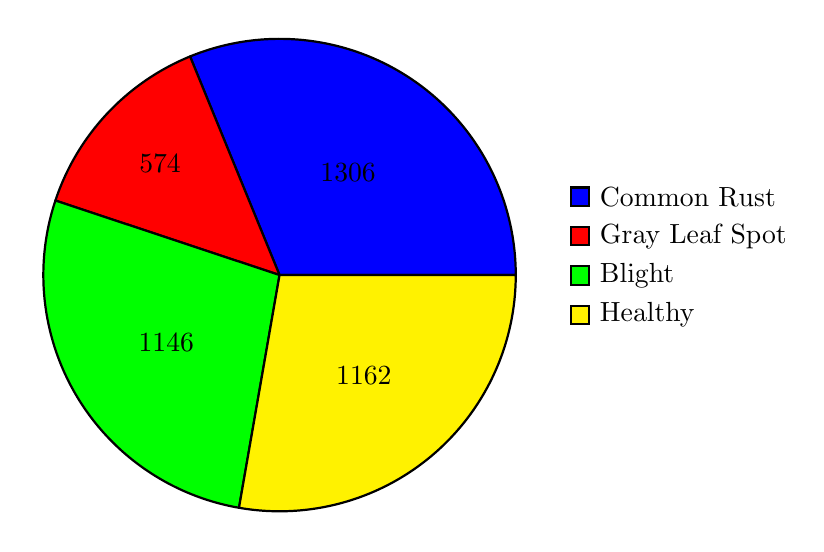
\begin{tikzpicture}
        \pie[sum=auto, text=legend, radius=3, color={blue, red, green, yellow}] {1306/Common Rust, 574/Gray Leaf Spot, 1146/Blight, 1162/Healthy}
    \end{tikzpicture}
    \caption{\centering Diagram Lingkaran untuk Jumlah Data pada Setiap Kategori}
    \label{fig:pie_chart}
\end{figure}

Berikut adalah penjelasan mengenai masing-masing kelas dalam dataset ini:

\begin{itemize}
    \item {\textit{Common Rust}}: Kelas ini mencakup gambar daun jagung yang terinfeksi oleh penyakit karat daun, yang disebabkan oleh jamur \textit{Puccinia sorghi} \cite{BROWN2002}. Penyakit ini mengakibatkan bercak-bercak coklat kemerahan di permukaan daun, dan daun yang terinfeksi biasanya menunjukkan tanda-tanda penguningan pada bagian tengah daun.
    \item {\textit{Gray Leaf Spot}}: Kelas ini berisi gambar daun jagung yang terkena penyakit bercak daun abu-abu, yang disebabkan oleh jamur \textit{Cercospora zeae-maydis} \cite{CERON2023}. Ciri-ciri daun yang terinfeksi adalah munculnya bercak abu-abu yang berujung hitam pada daun, yang dapat mengurangi efisiensi fotosintesis pada tanaman.
    \item {\textit{Blight}}: Kelas ini terdiri dari gambar daun yang terinfeksi oleh penyakit hawar daun, yang dapat disebabkan oleh berbagai patogen seperti jamur atau bakteri. Penyakit ini menyebabkan daun jagung menguning, mati, dan mengering, yang dapat merusak jaringan daun secara luas \cite{JAKHAR2023}.
    \item {\textit{Healthy}}: Kelas ini mencakup gambar daun jagung yang tidak terinfeksi penyakit apapun, yang terlihat segar dan berwarna hijau normal. Daun jagung sehat memiliki tekstur yang tidak rusak dan tidak menunjukkan tanda-tanda kerusakan atau infeksi.
\end{itemize}

\subsection{Algoritma atau Model}
\begin{itemize}
    \item {\textbf{YOLOv8}}: \\
   \hspace*{2em}YOLOv8 yang dirilis pada Januari 2023 oleh Ultralytics, menawarkan berbagai versi skala untuk deteksi objek, mulai dari YOLOv8n (nano) hingga YOLOv8x (extra-large). Arsitekturnya mirip dengan YOLOv5, namun mengganti CSPLayer dengan modul C2f (cross-stage partial bottleneck dengan dua konvolusi) untuk meningkatkan akurasi deteksi. YOLOv8 mengadopsi model tanpa anchor dengan head yang dipisah untuk menangani tugas objectness, classification, dan regression secara mandiri, yang berkontribusi pada peningkatan akurasi model secara keseluruhan. Dengan kecepatan dan efisiensi yang tinggi, YOLOv8 menjadi model yang sangat andal dalam deteksi objek \cite{Terven2023}. Berikut penjelasan lengkap dari arsitektur YoloV8.
    \begin{figure}[H]
        \centering
        \includegraphics[width=0.9\textwidth]{Images/yolov8.png}
        \caption{\centering Arsitektur YoloV8 \cite{Terven2023}}
        \label{fig:activity-upload-gambar}
    \end{figure}
\begin{enumerate}
    \item \textbf{Backbone} \\
    \hspace*{2em}Backbone merupakan bagian pertama dalam arsitektur YOLOv8 yang bertanggung jawab untuk mengekstraksi fitur utama dari input gambar. Proses ini mencakup penurunan resolusi gambar secara bertahap untuk menghasilkan representasi fitur yang lebih mendalam dan kompleks, sambil meningkatkan jumlah channel untuk memperkaya informasi. Backbone terdiri dari dua bagian utama, yaitu Stem Layer dan Stage Layers.
    
    \hspace*{2em}Pada bagian Stem Layer, YOLOv8 memanfaatkan tiga lapisan ConvModule yang dirancang untuk memproses gambar awal yang berukuran 640x640x3. Setiap ConvModule terdiri dari operasi konvolusi 2D untuk menangkap pola fitur dasar, batch normalization untuk menstabilkan distribusi output, dan fungsi aktivasi SiLU untuk menambahkan non-linearitas. Lapisan ini secara bertahap mengurangi resolusi gambar sambil meningkatkan jumlah channel fitur hingga menghasilkan keluaran berukuran 320x320x64.
    
    \hspace*{2em}Setelah melewati Stem Layer, Backbone melanjutkan proses melalui empat Stage Layers. Pada Stage Layer 1, model menggunakan CSPResLayer untuk menangkap fitur pada resolusi tinggi dengan jumlah channel sebesar 128, menghasilkan keluaran berukuran 160x160x128. Di tahap berikutnya, yaitu Stage Layer 2, resolusi gambar kembali dikurangi menjadi 80x80, sementara jumlah channel meningkat menjadi 256. Proses ini terus berlangsung hingga Stage Layer 4, di mana ukuran keluaran akhir Backbone adalah 20x20x1024. Progresi ini memastikan bahwa Backbone menangkap fitur dari berbagai tingkat resolusi, mulai dari detail lokal hingga pola global yang kompleks.

    \item \textbf{Neck} \\
    \hspace*{2em}Setelah fitur diekstraksi oleh Backbone, bagian Neck bertugas untuk menggabungkan informasi fitur dari berbagai tingkat resolusi. Hal ini bertujuan untuk memperkuat kemampuan deteksi multi-skala, sehingga YOLOv8 dapat mendeteksi objek kecil, sedang, maupun besar dengan akurat. Neck dirancang dengan dua jalur utama, yaitu Top-Down Path dan Bottom-Up Path.
    
    \hspace*{2em}Pada jalur Top-Down Path, fitur yang dihasilkan oleh Backbone pada resolusi rendah, seperti 20x20x1024, di-upsample menjadi resolusi yang lebih tinggi, misalnya 40x40x512. Proses upsampling ini memungkinkan penggabungan fitur dari resolusi rendah dengan fitur dari Backbone yang memiliki resolusi lebih tinggi, seperti 40x40x512. Setelah resolusi fitur diselaraskan, operasi concatenation dilakukan untuk mengintegrasikan informasi dari kedua skala. Hasil penggabungan ini kemudian diproses lebih lanjut menggunakan ConvModule untuk menyelaraskan jumlah channel dan memperbaiki kualitas fitur. Sebagai langkah tambahan, CSPResLayer digunakan untuk menonjolkan fitur yang penting, dengan memanfaatkan mekanisme residual yang membantu mempertahankan informasi awal.
    
    \hspace*{2em}Selain jalur Top-Down Path, Neck juga mencakup jalur Bottom-Up Path yang bekerja dengan menyusun ulang fitur ke resolusi yang lebih rendah. Tujuan jalur ini adalah memastikan bahwa fitur dari skala besar dan kecil diproses bersama-sama untuk mendukung deteksi objek dengan ukuran yang bervariasi.

    \item \textbf{Head} \\
    \hspace*{2em}Bagian terakhir dari YOLOv8 adalah Head, yang bertugas menghasilkan prediksi akhir, termasuk regresi bounding box, klasifikasi objek, dan confidence score. Pada bagian ini, YOLOv8 menggunakan PPYOLOE Layer yang didukung oleh blok RepVGGBlock. PPYOLOE Layer bertanggung jawab memproses fitur dari Neck dengan efisiensi tinggi, sekaligus menyelaraskan fitur untuk mempersiapkan tahap akhir prediksi.
    
    \hspace*{2em}Pada tahap prediksi, Head menggunakan dua lapisan Conv2D. Lapisan pertama digunakan untuk menghasilkan prediksi klasifikasi objek, sementara lapisan kedua bertugas melakukan regresi bounding box. Setiap fitur dari berbagai resolusi, seperti P3, P4, dan P5, diproses secara terpisah untuk memastikan bahwa prediksi dilakukan dengan mempertimbangkan skala resolusi yang sesuai. Desain ini memungkinkan YOLOv8 mendeteksi objek dari berbagai ukuran dengan lebih akurat. Salah satu keunggulan Head YOLOv8 adalah pendekatan anchor-free-nya, yang menyederhanakan proses pelatihan dan meningkatkan efisiensi.
\end{enumerate}

   
  
    \item {\textbf{Penggunaan SAHI dalam Model}}\\
    \hspace*{2em}Slicing Aided Hyper Inference (SAHI) menggunakan teknik pemotongan selama proses inferensi \cite{AKYON2022}. Gambar asli \( I \) dibagi menjadi beberapa potongan tumpang tindih dengan ukuran \( M \times N \), yang disebut \( P_{I1}, P_{I2}, \dots, P_{Il} \). Setiap potongan kemudian diubah ukurannya dengan menjaga rasio aspek gambar. Setelah itu, deteksi objek dilakukan pada setiap potongan secara terpisah. Jika diperlukan, full-inference (FI) juga bisa dilakukan dengan gambar asli untuk mendeteksi objek yang lebih besar. Hasil prediksi dari potongan-potongan ini dan, jika ada, hasil FI digabungkan kembali ke dalam gambar asli menggunakan teknik Non-Maximum Suppression (NMS). Pada NMS, kotak yang memiliki nilai Intersection over Union (IoU) lebih besar dari ambang batas yang ditentukan \( T_m \) akan dipadankan, dan deteksi dengan probabilitas di bawah ambang batas \( T_d \) akan dihapus.

    
\end{itemize}

\subsection{Pra-Pelatihan (Prosedur)}
Aplikasi Roboflow digunakan untuk melakukan anotasi pada data untuk menandai semua jenis penyakit berdasarkan 3 kategori yang telah ditentukan. Kemudian, data yang telah dianotasi diproses terlebih dahulu sebelum digunakan dalam pelatihan model. Berikut adalah prosesnya:
\begin{itemize}
    \item \textbf{Pra-pemrosesan} 
    \begin{itemize}
    \item \textbf{Auto-Orient} \\
    Pengaturan ini secara otomatis memperbaiki orientasi gambar berdasarkan metadata, memastikan semua gambar memiliki orientasi yang konsisten.

    \item \textbf{Resize} \\
      Setiap gambar diubah ukurannya menjadi 640 x 640 piksel. Ukuran ini diperlukan untuk melatih model YOLOv8.
    \end{itemize}

     \item \textbf{Pembagian Data} \\
       Data yang telah melalui pra-pemrosesan akan dibagi menjadi tiga kategori, yaitu data latih, data uji, dan data evaluasi, dengan proporsi masing-masing sebesar 80:10:10. Pembagian ini dilakukan agar model dapat dilatih, divalidasi, dan diuji secara menyeluruh. Pembagian data tersebut adalah sebagai berikut:

        \begin{itemize}
            \item \textbf{Data Latih (80\%)}: Digunakan untuk melatih model agar dapat mengenali pola dan karakteristik pada gambar daun jagung berdasarkan kategori penyakitnya.
            \item \textbf{Data Uji (10\%)}: Digunakan untuk mengevaluasi performa model selama proses pengembangan guna memastikan model tidak mengalami overfitting atau underfitting.
            \item \textbf{Data Evaluasi (10\%)}: Digunakan sebagai tes akhir untuk mengukur performa model secara independen pada data yang belum pernah dilihat sebelumnya, memastikan akurasi prediksi yang baik pada data nyata.
        \end{itemize}
    
     \item \textbf{Augmentasi}  \\
     Augmentasi gambar hanya dilakukan pada data kategori latih (train). Langkah ini diambil untuk meningkatkan jumlah dan variasi data latih, sehingga model dapat belajar dari lebih banyak contoh yang berbeda. Dengan cara ini, model dapat menjadi lebih robust dan lebih mampu mengenali pola pada data yang lebih beragam, tanpa perlu mengubah data uji atau evaluasi yang harus tetap representatif terhadap kondisi data yang sesungguhnya.

    \begin{itemize}
    \item \textbf{Hue} \\
    Menyesuaikan hue setiap gambar secara acak dalam rentang -15 hingga +15 derajat. Ini mensimulasikan variasi warna kecil untuk membuat model lebih kuat terhadap perubahan warna.

    \item \textbf{Saturation} \\
    Mengubah saturasi setiap gambar dalam rentang -30\% hingga +30\%. Ini mengubah intensitas warna, membantu model beradaptasi dengan gambar yang memiliki kecerahan warna yang berbeda.

    \item \textbf{Brightness} \\
    Mengubah kecerahan setiap gambar dengan menyesuaikannya secara acak antara -23\% hingga +23\%. Ini membantu model belajar menangani gambar dengan kondisi pencahayaan yang berbeda.

    \item \textbf{Exposure} \\
    Mengubah eksposur setiap gambar dalam rentang -10\% hingga +10\%, mensimulasikan berbagai lingkungan pencahayaan untuk meningkatkan adaptabilitas model terhadap tingkat eksposur yang berbeda.

    \item \textbf{Blur} \\
    Menambahkan efek blur dengan radius maksimum 2.2 piksel. Ini meniru gambar yang tidak fokus atau blur karena gerakan, yang dapat membuat model lebih tahan terhadap sedikit keburaman pada data input.

    \item \textbf{Bounding Box: Flip (Horizontal)} \\
    Pengaturan ini membalik gambar dan anotasi bounding box secara horizontal. Augmentasi ini memberikan pandangan cermin objek, meningkatkan kemampuan model untuk mengenali fitur dari berbagai perspektif.
    \end{itemize}

   
\end{itemize}

\subsection{Metrik Evaluasi}
\begin{itemize}
    \item \textbf{Box Loss} \\
    Model YOLO yang dikembangkan oleh Ultralytics menggunakan Complete Intersection Over Union (CIoU) untuk menilai seberapa baik prediksi bounding box cocok dengan bounding box target dalam tugas deteksi objek\cite{Smith2023}. Berikut adalah Persamaan CIoU:
    
    \[
    \text{CIoU}(A, B) = 1 - \text{IoU}(A, B) + \frac{\rho^2(\mathbf{b}, \mathbf{b}^g)}{c^2} + \alpha v
    \]
    
    Keterangan:
    \begin{itemize}
        \setlength{\itemindent}{1em} % Menambahkan indentasi untuk bullet point
        \item \( \text{IoU}(A, B) \) adalah Intersection over Union antara bounding box \( A \) dan \( B \).
        \item \( \rho(\mathbf{b}, \mathbf{b}^g) \) adalah jarak Euklidean antara pusat dari bounding box prediksi \( \mathbf{b} \) dan bounding box target \( \mathbf{b}^g \).
        \item \( c \) adalah diagonal dari kotak yang mengelilingi kedua bounding box.
        \item \( \alpha \) dan \( v \) adalah parameter penyeimbang untuk aspek rasio.
    \end{itemize}

    \item \textbf{Class Loss} \\
    Classification Loss (class loss atau cls loss) dalam YOLOv8 mengukur seberapa akurat model dalam mengklasifikasikan objek yang terdeteksi ke dalam kelas yang benar. Ini dilakukan dengan membandingkan probabilitas kelas yang diprediksi model dengan kelas yang sebenarnya (ground truth). Cross-Entropy Loss digunakan dalam perhitungan class loss\cite{Encord2023}. Berikut adalah Persamaan Cross-Entropy Loss:
    
    \[
        L_{\text{cls}} = - \sum_{c=1}^{C} y_c \log(p_c)
    \]
    
    Keterangan:
    \begin{itemize}
        \setlength{\itemindent}{1em} % Menambahkan indentasi untuk bullet point
        \item \( C \) adalah jumlah kelas dalam dataset (misalnya, jumlah kelas objek yang perlu dideteksi).
        \item \( y_c \) adalah label kelas target (nilai 1 jika objek termasuk dalam kelas \( c \), atau 0 jika tidak).
        \item \( p_c \) adalah probabilitas prediksi untuk kelas \( c \), yang dihitung oleh model.
    \end{itemize}

     \item \textbf{Precision} \\
    Precision mengukur seberapa banyak prediksi positif model yang benar. Ini dihitung dengan membandingkan jumlah deteksi yang benar dengan total deteksi yang dilakukan. Precision memberikan informasi tentang seberapa tepat model dalam memprediksi objek, yang penting untuk mengevaluasi apakah model menghasilkan banyak prediksi yang salah atau tidak\cite{Zhang2021}. Berikut adalah Persamaan Precision:
    
    \[
        \text{Precision} = \frac{TP}{TP + FP}
    \]
    
    Keterangan:
    \begin{itemize}
        \setlength{\itemindent}{1em} % Menambahkan indentasi untuk bullet point
        \item \( TP \) adalah jumlah \textit{True Positives} (prediksi benar yang cocok dengan ground truth).
         \item \( FP \) adalah jumlah \textit{False Positives} (prediksi salah).
    \end{itemize}
    

    \item \textbf{Recall} \\
    Recall mengukur seberapa banyak objek yang benar-benar ada dalam gambar yang berhasil dideteksi oleh model. Recall memberikan informasi tentang seberapa baik model dalam menemukan objek yang ada dalam gambar, yang penting untuk mengevaluasi kemampuan model dalam mendeteksi semua objek yang relevan\cite{Zhang2021}. Berikut adalah Persamaan Recall:
    
    \[
        \text{Recall} = \frac{TP}{TP + FN}
    \]
    
    Keterangan:
    \begin{itemize}
        \setlength{\itemindent}{1em} % Menambahkan indentasi untuk bullet point
         \item \( TP \) adalah jumlah \textit{True Positives} (prediksi benar yang cocok dengan ground truth).
    \item \( FN \) adalah jumlah \textit{False Negatives} (objek yang ada namun tidak terdeteksi oleh model).
    \end{itemize}

    \item \textbf{mAP50} \\
    Mean Average Precision pada threshold Intersection over Union (IoU) 0.5 (\textit{mAP@50}) adalah rata-rata dari \textit{average precision} (AP) pada berbagai kategori objek untuk IoU lebih dari 50\%. Metrik ini digunakan untuk mengevaluasi seberapa baik model dalam mendeteksi objek secara keseluruhan, dengan fokus pada deteksi yang tepat, mengabaikan deteksi yang tidak sesuai dengan objek yang sebenarnya\cite{Zhang2021}. Berikut adalah Persamaan mAP50:
    
    \[
        \text{mAP@50} = \frac{1}{N} \sum_{i=1}^{N} \text{AP@50}_i
    \]
    
    Keterangan:
    \begin{itemize}
        \setlength{\itemindent}{1em} % Menambahkan indentasi untuk bullet point
       \item \( N \) adalah jumlah kategori objek dalam dataset.
    \item \( \text{AP@50}_i \) adalah \textit{Average Precision} pada kategori ke-\( i \) dengan threshold IoU 0.5.
    \end{itemize}

    \item \textbf{mAP50-95} \\
    Mean Average Precision pada IoU thresholds dari 0.5 hingga 0.95, dengan interval 0.05. Metrik ini memberikan gambaran yang lebih mendetail tentang performa model dalam mendeteksi objek pada berbagai tingkat overlap. Dengan menghitung precision pada berbagai threshold, mAP@50-95 memberikan evaluasi yang lebih komprehensif mengenai kemampuan model dalam mengidentifikasi objek pada berbagai tingkat ketepatan prediksi\cite{Zhang2021}.
    Berikut adalah Persamaan mAP50-95:
    
    \[
      \text{mAP@50-95} = \frac{1}{N} \sum_{i=1}^{N} \text{AP@thresholds}_i
    \]

    
    Keterangan:
    \begin{itemize}
        \setlength{\itemindent}{1em} % Menambahkan indentasi untuk bullet point
          \item \( N \) adalah jumlah kategori objek.
    \item \( \text{AP@thresholds}_i \) adalah average precision untuk kategori ke-\( i \) pada berbagai nilai threshold IoU dari 0.5 hingga 0.95 dengan interval 0.05.
    \end{itemize}

    

\end{itemize}


%%%%%%%%%%%%%%%%%%%%%%%%%%%%%%%%%%%%%%%%%%
\section{Sistem Kecerdasan}
Sistem kecerdasan pada aplikasi \textit{LeafScan} didasarkan pada penerapan teknologi \textit{deep learning} untuk mendeteksi penyakit pada daun jagung secara otomatis melalui gambar yang diunggah oleh pengguna. Sistem ini memanfaatkan model \textit{You Only Look Once} v8 (YOLOv8) yang dikombinasikan dengan algoritma \textit{Slicing Aided Hyper Inference} (SAHI) untuk meningkatkan akurasi dan efisiensi deteksi objek. YOLOv8, yang dikenal dengan kemampuannya untuk mendeteksi objek \cite{YIN2020}, digunakan untuk mendeteksi penyakit pada daun jagung. Sementara itu, SAHI membantu dalam meningkatkan kemampuan model dalam menangani gambar dengan objek yang lebih kecil atau lebih kompleks, serta meningkatkan akurasi prediksi dengan melakukan pemotongan gambar untuk memaksimalkan deteksi \cite{AKYON2022}.

\subsection{Arsitektur Sistem}

Arsitektur sistem \textit{LeafScan} dirancang untuk mengoptimalkan deteksi penyakit pada daun jagung dengan menggunakan berbagai teknologi modern yang terintegrasi. Terdapat tiga elemen utama dalam arsitektur ini, yaitu \textit{Frontend}, \textit{Back-End}, dan \textit{Storage}.

% Gambar Arsitektur Sistem
\begin{figure}[H]
    \centering
    \includegraphics[width=0.8\textwidth]{Images/architecture_system.png}
    \caption{\centering Arsitektur Sistem \textit{LeafScan}}
    \label{fig:arsitektur-sistem}
\end{figure}

\begin{itemize}
    \item \textbf{\textit{Frontend}} \\
    Frontend aplikasi \textit{LeafScan} dikembangkan menggunakan \textit{Flutter}, yang memungkinkan pembuatan aplikasi mobile yang responsif dan dapat dijalankan di berbagai platform seperti Android dan iOS \cite{ALANAZI2024}. Flutter menyediakan antarmuka pengguna yang interaktif dan mudah digunakan, memungkinkan pengguna untuk mengunggah gambar daun jagung yang ingin dideteksi penyakitnya. Pengguna dapat melihat hasil deteksi serta rekomendasi pengobatan yang dihasilkan oleh sistem.
    
    \item \textbf{\textit{Back-End}} \\
    \textit{Google Compute Engine} digunakan sebagai server untuk menjalankan model deep learning YOLOv8 yang diintegrasikan dengan algoritma \textit{Slicing Aided Hyper Inference} (SAHI). Model ini berfungsi untuk menganalisis gambar daun jagung yang diunggah dan mendeteksi kemungkinan adanya penyakit. \textit{Google Compute Engine} memberikan infrastruktur yang skalabel dan dapat menangani permintaan pengguna secara efisien, sehingga memastikan proses deteksi berjalan dengan cepat dan akurat \cite{VOLKOV2017}. Selain itu, sistem juga mengintegrasikan \textit{API GPT} yaitu \textit{OpenAI GPT} untuk memberikan rekomendasi berbasis teks yang lebih spesifik sesuai dengan jenis penyakit yang terdeteksi pada daun jagung. \textit{API GPT} dapat membantu menyediakan informasi tambahan mengenai cara pengobatan dan pencegahan penyakit bagi petani.
    
    \item \textbf{\textit{Storage}} \\
    \textit{Google Cloud Storage} (GCP) digunakan untuk menyimpan data deteksi, termasuk gambar yang diunggah oleh pengguna dan hasil deteksi penyakit. Penyimpanan cloud ini memastikan data dapat diakses secara efisien dan aman dari berbagai perangkat. GCP juga memudahkan pengelolaan data dalam jumlah besar dan mendukung skalabilitas sistem \cite{LICHTENTDAHL2023}. Selain itu, \textit{Firebase} digunakan untuk mengelola autentikasi pengguna, memungkinkan pengguna untuk mendaftar dan masuk ke aplikasi dengan aman \cite{MARTINS2024}. Dengan \textit{Firebase}, data pengguna seperti riwayat deteksi dan rekomendasi pengobatan juga dapat disinkronkan dengan mudah dan memberikan kenyamanan lebih bagi pengguna yang ingin mengakses data mereka kapan saja.
\end{itemize}

\subsection{Alur Kerja Sistem}

Alur kerja sistem \textit{LeafScan} mencakup serangkaian proses yang dimulai dari pengguna mengunggah gambar daun jagung hingga mendapatkan hasil deteksi penyakit dan rekomendasi penanganan. Berikut ini adalah deskripsi dari diagram \textit{use case} dan \textit{activity diagram} yang merepresentasikan alur kerja aplikasi.

\subsubsection{Use Case Diagram}
Aplikasi \textit{LeafScan} memiliki beberapa aktor utama, yaitu Petani dan Mahasiswa Pertanian, yang memiliki akses ke berbagai fitur sistem. Berikut adalah penjelasan dari tiap \textit{use case}:

\begin{itemize}
    \item Mendeteksi Penyakit Daun Jagung: Aktor Petani dan Mahasiswa Pertanian dapat menggunakan aplikasi untuk mendeteksi penyakit pada daun jagung dengan mengunggah gambar daun yang akan dianalisis.
    \item Mengupload Gambar: Proses ini adalah bagian dari deteksi penyakit daun jagung. Pengguna perlu mengunggah gambar untuk menjalankan proses deteksi.
    \item Memberi Rekomendasi Penanganan: Jika penyakit terdeteksi, sistem akan memberikan rekomendasi penanganan yang sesuai.
    \item Melihat Riwayat Deteksi Penyakit: Aktor Petani dan Mahasiswa Pertanian dapat melihat riwayat deteksi penyakit yang telah dilakukan sebelumnya, sehingga memudahkan dalam memantau perkembangan kondisi daun jagung dari waktu ke waktu.
\end{itemize}

\begin{figure}[H]
    \centering
    \includegraphics[width=0.8\textwidth]{Images/use_case.png}
    \caption{\centering Diagram Use Case Aplikasi \textit{LeafScan}}
    \label{fig:use-case}
\end{figure}

\subsubsection{Activity Diagram}
Untuk memperjelas alur kerja aplikasi, berikut ini adalah \textit{activity diagram} yang menggambarkan proses utama dari saat pengguna memulai interaksi hingga mendapatkan rekomendasi penanganan penyakit.

\begin{enumerate}[label=\alph*)]
    \item \textbf{Activity Diagram - Mengupload Gambar} \\
    Pada Gambar \ref{fig:activity-upload-gambar}, diperlihatkan alur aktivitas untuk proses Mengupload Gambar. Proses ini dimulai ketika pengguna menekan tombol untuk deteksi gambar dan memilih opsi pengambilan gambar dari kamera atau galeri. Setelah gambar diambil, pengguna dapat memotong gambar sebelum mengunggahnya ke server. Sistem kemudian menampilkan konfirmasi upload dan melanjutkan untuk mengunggah gambar ke server.
    
    \begin{figure}[H]
        \centering
        \includegraphics[width=0.5\textwidth]{Images/activity_upload.png}
        \caption{\centering Diagram Aktivitas untuk Mengupload Gambar}
        \label{fig:activity-upload-gambar}
    \end{figure}

    \item \textbf{Activity Diagram - Mendeteksi Penyakit Daun Jagung} \\
    Pada Gambar \ref{fig:activity-detect-disease}, diperlihatkan alur aktivitas untuk proses mendeteksi penyakit daun jagung. Setelah pengguna mengunggah gambar, sistem menggunakan model \textit{deep learning} (YOLOv8) untuk melakukan deteksi penyakit pada daun jagung. Setelah analisis selesai, hasil deteksi akan ditampilkan kepada pengguna.

    % Uncomment and add the appropriate figure if you have an activity diagram for detecting diseases
    \begin{figure}[H]
        \centering
        \includegraphics[width=0.5\textwidth]{Images/activity_detect.png}
        \caption{\centering Diagram Aktivitas untuk Mendeteksi Penyakit Daun Jagung}
        \label{fig:activity-detect-disease}
    \end{figure}
    
    \item \textbf{Activity Diagram - Memberi Rekomendasi Penanganan} \\
    Pada Gambar \ref{fig:activity-rekomendasi-penanganan}, dijelaskan proses aktivitas untuk Memberi Rekomendasi Penanganan. Setelah sistem mendapatkan hasil deteksi, jenis penyakit diidentifikasi, dan sistem menampilkan informasi lengkap tentang penyakit. Selanjutnya, sistem memberikan daftar rekomendasi penanganan. Pengguna dapat memilih rekomendasi yang sesuai, dan sistem menampilkan rincian lebih lanjut mengenai tindakan penanganan yang disarankan.
    
    \begin{figure}[H]
        \centering
        \includegraphics[width=0.5\textwidth]{Images/activity_recomendation.png}
        \caption{\centering Diagram Aktivitas untuk Memberi Rekomendasi Penanganan}
        \label{fig:activity-rekomendasi-penanganan}
    \end{figure}

    \item \textbf{Activity Diagram - Melihat Riwayat Deteksi Penyakit} \\
    Pada Gambar \ref{fig:activity-view-history1}, diperlihatkan alur aktivitas untuk proses \textit{Melihat Riwayat Deteksi Penyakit}. Proses ini dimulai dengan sistem menampilkan daftar riwayat penyakit yang telah terdeteksi sebelumnya. Pengguna kemudian dapat memilih salah satu riwayat deteksi dari daftar untuk melihat lebih detail. Setelah riwayat dipilih, sistem menampilkan informasi rinci tentang hasil deteksi dan rekomendasi penanganan yang telah diberikan sebelumnya.
    
    \begin{figure}[H]
        \centering
        \includegraphics[width=0.5\textwidth]{Images/activity_history.png}
        \caption{\centering Diagram Aktivitas untuk Melihat Riwayat Deteksi Penyakit}
        \label{fig:activity-view-history1}
    \end{figure}
\end{enumerate}
%%%%%%%%%%%%%%%%%%%%%%%%%%%%%%%%%%%%%%%%%%

\section{Hasil}
\subsection{Hasil Training}
\begin{itemize}
    \item {\textbf{Grafik Training}}: \\ 
      \hspace*{2em}Grafik ini menunjukkan berbagai metrik dan loss selama proses pelatihan model. 
        Grafik pada baris pertama menampilkan \textit{train/box\_loss}, \textit{train/cls\_loss}, dan \textit{train/obj\_loss}, yang semuanya menunjukkan tren penurunan seiring dengan meningkatnya jumlah epoch, menandakan bahwa model semakin baik dalam mempelajari data pelatihan. 
        Baris kedua memperlihatkan metrik untuk data validasi, seperti \textit{val/box\_loss}, \textit{val/cls\_loss}, dan \textit{val/obj\_loss}, yang juga menunjukkan penurunan. 
        Selain itu, metrik performa seperti \textit{precision}, \textit{recall}, \textit{mAP@0.5}, dan \textit{mAP@0.5:0.95} cenderung meningkat dan stabil di akhir pelatihan, menandakan peningkatan kemampuan model dalam mendeteksi dan mengenali objek dengan lebih akurat.
    \begin{figure}[H]
        \centering
        \includegraphics[width=0.8\textwidth]{Images/results.png}
        \caption{\centering Diagram Aktivitas untuk Melihat Riwayat Deteksi Penyakit}
        \label{fig:activity-view-history}
    \end{figure}
    \item {\textbf{Precision}}: \\ 
       \hspace*{2em}Grafik ini menunjukkan hubungan antara precision (akurasi prediksi model dalam mendeteksi suatu kelas) dan confidence (tingkat keyakinan model pada prediksi yang dibuat), di mana precision yang tinggi menunjukkan prediksi model lebih tepat pada tingkat confidence tertentu. Pada grafik ini, kelas blight memiliki kurva precision yang tinggi pada confidence sekitar 0.6 hingga 1.0, menunjukkan performa yang baik dalam mendeteksi kelas ini, sementara kelas rust memiliki kurva precision yang lebih rendah, menandakan performa model yang buruk untuk mendeteksi kelas tersebut di sebagian besar tingkat confidence. Kurva all classes menggambarkan hasil gabungan dari semua kelas yang terlibat dalam evaluasi.
    \begin{figure}[H]
        \centering
        \includegraphics[width=0.7\textwidth]{Images/P_curve.png}
        \caption{\centering Grafik menggambarkan nilai precision selama pelatihan model YOLOv8}
        \label{fig:activity-view-history}
    \end{figure}
    \item {\textbf{Recall}}: \\ 
    \hspace*{2em}Grafik ini menggambarkan hubungan antara recall (kemampuan model untuk mendeteksi semua instance dari suatu kelas) dan confidence, di mana recall yang tinggi menunjukkan model mampu mendeteksi sebagian besar instance dari kelas tersebut. Pada grafik ini, kelas blight memiliki recall yang lebih stabil, meskipun cenderung menurun pada tingkat confidence yang lebih tinggi, sedangkan kelas rust memiliki recall yang rendah, menunjukkan bahwa model kesulitan mendeteksi instance dari kelas ini secara keseluruhan.
    \begin{figure}[H]
        \centering
        \includegraphics[width=0.7\textwidth]{Images/R_curve.png}
        \caption{\centering Grafik menggambarkan nilai recall selama pelatihan model YOLOv8}
        \label{fig:activity-view-history}
    \end{figure}
\end{itemize}

\subsection{Perkembangan Aplikasi LeafScan}
Berikut ini adalah deskripsi dari masing-masing bagian \textit{frontend} dan \textit{backend} yang telah dikerjakan:

\begin{itemize}
    \item \textbf{Frontend} \\
    Pengembangan \textit{frontend} aplikasi \textit{LeafScan} menggunakan \textit{framework Flutter} untuk menciptakan antarmuka yang intuitif dan responsif. Beberapa fitur \textit{frontend} yang sudah dikerjakan antara lain:

     \begin{itemize}
        \begin{figure}[H]
            \centering
            \begin{minipage}{0.3\textwidth}
                \centering
                \includegraphics[width=0.8\textwidth]{Images/login_view.png}
                \caption{\centering Tampilan Login}
                \label{fig:login-view}
            \end{minipage}
            \hfill
            \begin{minipage}{0.3\textwidth}
                \centering
                \includegraphics[width=0.8\textwidth]{Images/register_view.png}
                \caption{\centering Tampilan Register}
                \label{fig:register-view}
            \end{minipage}
            \hfill
            \begin{minipage}{0.3\textwidth}
                \centering
                \includegraphics[width=0.8\textwidth]{Images/daun_sehat.png}
                \caption{\centering Tampilan Daun Sehat}
                \label{fig:register-view}
            \end{minipage}
        \end{figure}
        
        \begin{figure}[H]
            \centering
            \begin{minipage}{0.3\textwidth}
                \centering
                \includegraphics[width=0.9\textwidth]{Images/hasil_deteksi.png}
                \caption{Tampilan Hasil Deteksi}
                \label{fig:detection-view}
           \end{minipage}
            \hfill
            \begin{minipage}{0.3\textwidth}
                \centering
                \includegraphics[width=0.9\textwidth]{Images/detail_penyakit.png}
                \caption{Tampilan Detail Penyakit}
                \label{fig:detail-disease-view}
            \end{minipage}
            \hfill
            \begin{minipage}{0.3\textwidth}
                \centering
                \includegraphics[width=0.9\textwidth]{Images/history_view.png}
                \caption{Tampilan Riwayat Deteksi}
                \label{fig:history-view}
            \end{minipage}
            \label{fig:combined-views}
        \end{figure}

        \begin{figure}[H]
            \centering
            \begin{minipage}{0.4\textwidth}
                \centering
                \includegraphics[width=0.9\textwidth]{Images/not_leaf.png}
                \caption{\centering Tampilan Deteksi Bukan Daun}
                \label{fig:not-leaf}
           \end{minipage}
            \hfill
            \begin{minipage}{0.4\textwidth}
                \centering
                \includegraphics[width=0.9\textwidth]{Images/splash screen.jpeg}
                \caption{\centering Splash Screen}
                \label{fig:splash-screen}
            \end{minipage}
        \end{figure}
    \end{itemize}

    \item \textbf{Backend} \\
    Pengembangan \textit{backend} aplikasi \textit{LeafScan} dilakukan untuk mendukung proses deteksi penyakit dan penyimpanan data secara efisien. Berikut komponen \textit{backend} yang sudah dikerjakan yaitu:

    \textbf{- Dokumentasi API}

    \begin{itemize}[left=0pt, label={}]
        \item \textbf{URL:} \texttt{/predict-image}
        \item \textbf{Method:} \texttt{POST}
        \item \textbf{Request Parameters:}
        \begin{itemize}
            \item \texttt{file} (\textit{required}): Berkas gambar yang digunakan untuk mendeteksi penyakit daun jagung. \\
            \textit{Format yang didukung}: JPEG, PNG.
        \end{itemize}
    
        \item \textbf{Response:}
        \begin{itemize}
            \item \texttt{disease}: Kamus yang berisi detail tentang berbagai penyakit daun jagung:
            \begin{itemize}
                \item \texttt{gray}:
                \begin{itemize}
                    \item \texttt{Definisi}: Deskripsi singkat mengenai penyakit ini.
                    \item \texttt{Diagnosa}: Tanda-tanda diagnostik penyakit.
                    \item \texttt{Saran}: Tindakan atau solusi yang disarankan.
                \end{itemize}
                \item \texttt{rust}:
                \begin{itemize}
                    \item \texttt{Definisi}: Deskripsi singkat mengenai penyakit ini.
                    \item \texttt{Diagnosa}: Tanda-tanda diagnostik penyakit.
                    \item \texttt{Saran}: Tindakan atau solusi yang disarankan.
                \end{itemize}
                \item \texttt{blight}:
                \begin{itemize}
                    \item \texttt{Definisi}: Deskripsi singkat mengenai penyakit ini.
                    \item \texttt{Diagnosa}: Tanda-tanda diagnostik penyakit.
                    \item \texttt{Saran}: Tindakan atau solusi yang disarankan.
                \end{itemize}
            \end{itemize}
            \item \texttt{status\_code} (integer): Kode status HTTP dari permintaan.
            \item \texttt{predicted\_image} (string): String gambar hasil prediksi dalam format Base64.
            \item \texttt{timestamp} (string): Waktu kapan prediksi dilakukan.
            \item \texttt{iscorn} (boolean): Menunjukkan apakah gambar teridentifikasi terkait jagung.
        \end{itemize}
    \end{itemize}
    \begin{figure}[H]
        \centering
        \includegraphics[width=0.5\textwidth]{Images/response json.png}
        \caption{\centering \textit{Response} pengujian API}
        \label{fig:apiEndpoint}
    \end{figure}
\end{itemize}
%%%%%%%%%%%%%%%%%%%%%%%%%%%%%%%%%%%%%%%%%%
\section{Diskusi}
\subsection{Implementasi SAHI dalam proses inferensi}
Berdasarkan hasil evaluasi model, terlihat bahwa objek penyakit berukuran kecil masih cukup sulit untuk dideteksi secara akurat. Hal ini disebabkan oleh keterbatasan model dalam mengenali detail-detail kecil pada gambar. Salah satu upaya yang telah dilakukan untuk mengatasi masalah ini adalah dengan menurunkan confidence threshold untuk meningkatkan probabilitas sebuah objek penyakit terdeteksi. Namun, pendekatan ini memiliki kelemahan, yaitu meningkatkan risiko terjadinya kesalahan prediksi (false positives), di mana model mendeteksi objek yang sebenarnya tidak ada.

Dalam mengatasi kelemahan ini, implementasi Slicing Aided Hyper Inference (SAHI) telah dilakukan. Teknik SAHI membantu model dalam melakukan proses inferensi dengan cara membagi gambar menjadi beberapa subset gambar yang lebih kecil (proses slicing). Dengan memperkecil skala tiap subset, SAHI dapat memperbesar ukuran relatif dari objek penyakit pada subset tersebut, sehingga model lebih mudah mengenalinya. Hasil evaluasi menunjukkan bahwa teknik ini secara signifikan meningkatkan kemampuan model dalam mendeteksi objek penyakit kecil, meskipun model tersebut belum sepenuhnya optimal.

Namun, penggunaan SAHI juga memiliki beberapa konsekuensi, salah satunya adalah peningkatan waktu proses inferensi. Hal ini terjadi karena proses slicing menghasilkan sejumlah besar subset gambar, yang jumlahnya berbanding lurus dengan ukuran asli gambar. Semakin besar ukuran gambar, semakin banyak subset yang dihasilkan, sehingga memerlukan waktu pemrosesan lebih lama.

 \begin{figure}[H]
            \centering
            \begin{minipage}{0.45\textwidth}
                \centering
                \includegraphics[width=0.8\textwidth]{Images/predicted_0.jpg}
                \caption{\centering Hasil Deteksi Model YoloV8 tanpa SAHI}
                \label{fig:login-view}
            \end{minipage}
            \hfill
            \begin{minipage}{0.45\textwidth}
                \centering
                \includegraphics[width=0.8\textwidth]{Images/predicted_sahi.png}
                \caption{\centering Hasil Deteksi Model YoloV8 setelah SAHI diimplementasikan}
                \label{fig:register-view}
            \end{minipage}
        \end{figure}
\section{Kesimpulan}
Penelitian ini bertujuan untuk mengukur akurasi diagnosis penyakit daun jagung yang dihasilkan oleh aplikasi \textit{LeafScan} dibandingkan metode manual. Hasil menunjukkan bahwa aplikasi berhasil memenuhi tujuan ini dengan model yang mampu mempelajari data pelatihan secara efektif, sebagaimana ditunjukkan oleh tren penurunan loss dan peningkatan \textit{precision}, \textit{recall}, serta mAP selama proses pelatihan dan validasi. Dengan demikian, \textit{LeafScan} berpotensi menjadi alat yang bermanfaat bagi petani dalam mendeteksi penyakit daun jagung dengan lebih cepat dan akurat.

Hasil evaluasi menunjukkan bahwa performa model cukup baik dalam mendeteksi kelas penyakit tertentu, seperti \textit{blight}, dengan \textit{precision} dan \textit{recall} yang tinggi pada tingkat \textit{confidence} antara 0.6 hingga 1.0. Namun, terdapat kelemahan dalam mendeteksi penyakit seperti \textit{rust} yang memiliki performa lebih rendah. Masalah ini terkait dengan kesulitan model dalam mengenali objek kecil. Implementasi teknik \textit{Slicing Aided Hyper Inference} (SAHI) secara signifikan meningkatkan deteksi objek kecil, tetapi diiringi oleh peningkatan waktu proses inferensi karena kebutuhan pemrosesan lebih banyak subset gambar.

Untuk pengembangan di masa depan, penelitian ini merekomendasikan optimalisasi teknik SAHI guna mengurangi waktu proses inferensi tanpa mengorbankan akurasi deteksi. Selain itu, pengembangan model yang lebih sensitif terhadap objek kecil atau integrasi model berbasis arsitektur yang lebih kompleks seperti \textit{transformers} dapat dipertimbangkan. Uji coba lapangan dengan melibatkan petani secara langsung juga perlu dilakukan untuk mengukur penerimaan aplikasi serta manfaatnya dalam kondisi nyata, sekaligus mendapatkan umpan balik untuk penyempurnaan aplikasi.
%=====================================
% References, variant A: external bibliography
%=====================================
%\bibliography{your_external_BibTeX_file}

%=====================================
% References, variant B: internal bibliography
%=====================================

\begin{adjustwidth}{-\extralength}{0cm}
% \printendnotes[custom] % Un-comment to print a list of endnotes

\reftitle{References}

% Please provide either the correct journal abbreviation (e.g. according to the “List of Title Word Abbreviations” http://www.issn.org/services/online-services/access-to-the-ltwa/) or the full name of the journal.
% Citations and References in Supplementary files are permitted provided that they also appear in the reference list here.

\begin{thebibliography}{999}
% Reference 1
\bibitem[Sari et al.(2023)]{Sari2023}
Sari, D.; Supriyadi, E. Identifikasi Penyakit Tanaman Jagung Berdasarkan Citra Daun Menggunakan Convolutional Neural Network. {\em Jurnal Pertanian Terapan} {\bf 2023}, {\em 22}(3), 45--56. DOI: \url{10.33633/tc.v22i3.8425}.
% Reference 2
\bibitem[Husni and Rahman(2023)]{Husni2023}
Husni, M.; Rahman, A. Application Development of Expert System for Early Detection of Pests and Diseases of Corn Plants. {\em Jurnal Pertanian Pangan dan Teknologi} {\bf 2023}, {\em 24}(1), 15--25. DOI: \url{10.25181/jppt.v24i1.3039}.
% Reference 3
\bibitem[Putra and Yulianto(2023)]{Putra2023}
Putra, R.; Yulianto, F. Corn Leaf Diseases Recognition Based on Convolutional Neural Network. {\em International Journal of Technology Research and Development} {\bf 2023}, {\em 12}(2), 67--78. DOI: \url{10.25299/itjrd.2023.13904}.
% Reference 4
\bibitem[Brown(2002)]{BROWN2002}
Brown, J. K. M. Yield Penalties of Disease Resistance in Crops. {\em Current Opinion in Plant Biology} {\bf 2002}, {\em 5}(4), 339--344. DOI: \url{https://doi.org/10.1016/S1369-5266(02)00270-4}.
% Reference 5
\bibitem[Cerón-Bustamante et al.(2023)]{CERON2023}
Cerón-Bustamante, M.; Balducci, E.; Beccari, G.; Nicholson, P.; Covarelli, L.; Benincasa, P. Effect of Light Spectra on Cereal Fungal Pathogens, a Review. {\em Fungal Biology Reviews} {\bf 2023}, {\em 43}, 100291. DOI: \url{https://doi.org/10.1016/j.fbr.2022.10.004}.
% Reference 6
\bibitem[Jakhar et al.(2023)]{JAKHAR2023}
Jakhar, D. S.; Kumari, R.; Kumar, P.; Singh, R.; Kumar, A. Chapter 16 - Exserohilum turcicum [Pass.] resistance in maize: A sustainable agricultural approach for studying plant-microbe interactions. In {\em Plant-Microbe Interaction - Recent Advances in Molecular and Biochemical Approaches}; Swapnil, P.; Meena, M.; Harish, ; Marwal, A.; Vijayalakshmi, S.; Zehra, A., Eds.; Academic Press: 2023; pp 363--373. DOI: \url{https://doi.org/10.1016/B978-0-323-91875-6.00016-5}.
% Reference 7
\bibitem[Yin et al.(2020)]{YIN2020}
Yin, Y.; Li, H.; Fu, W. Faster-YOLO: An accurate and faster object detection method. In {\em Digital Signal Processing}; 2020; Volume 102, 102756. DOI: \url{https://doi.org/10.1016/j.dsp.2020.102756}.
% Reference 8
\bibitem[Akyon et al.(2022)]{AKYON2022}
Akyon, F. C.; Altinuc, O.; Temizel, A. Slicing Aided Hyper Inference and Fine-Tuning for Small Object Detection. In {\em 2022 IEEE International Conference on Image Processing (ICIP)}; 2022; pp. 966-970. DOI: \url{https://doi.org/10.1109/ICIP46576.2022.9897990}.
% Reference 9
\bibitem[Alanazi and Alfayez(2024)]{ALANAZI2024}
Alanazi, A.; Alfayez, R. What is discussed about Flutter on Stack Overflow (SO) question-and-answer (Q\&A) website: An empirical study. In {\em Journal of Systems and Software}; 2024; Vol. 215, pp. 112089. DOI: \url{https://doi.org/10.1016/j.jss.2024.112089}.
% Reference 10
\bibitem[Volkov and Sukhoroslov(2017)]{VOLKOV2017}
Volkov, S.; Sukhoroslov, O. Simplifying the Use of Clouds for Scientific Computing with Everest. In {\em Procedia Computer Science}; 2017; Vol. 119, pp. 112-120. DOI: \url{https://doi.org/10.1016/j.procs.2017.11.167}.
% Reference 11
\bibitem[Lichtendahl et al.(2023)]{LICHTENTDAHL2023}
Lichtendahl, K. C.; Andrasko, J.; Boatright, B. Google Cloud Platform: Cloud Storage. In {\em Darden Case No. UVA-QA-0941}; 2023. Available at SSRN: \url{https://ssrn.com/abstract=4133739} or \url{http://dx.doi.org/10.2139/ssrn.4133739}.
% Reference 12
\bibitem[Martins et al.(2024)]{MARTINS2024}
Martins, P.; Jorge, H.; Aidos, M.; Cristovam, R.; Váz, P.; Silva, J.; Abbasi, M. Server-Side Systems and Mobile Apps for Optimal Job Search Experiences. In {\em Procedia Computer Science}; 2024; {\bf 238}, pp. 587-593. DOI: \url{https://doi.org/10.1016/j.procs.2024.06.065}.
% Reference 13
\bibitem[Zhang et al.(2021)]{Zhang2021}
Zhang, Y.; Wang, X.; Li, Z. Survey and Performance Analysis of Deep Learning Based Object Detection in Challenging Environments. {\em Sensors} {\bf 2021}, {\em 21}(15), 5116. DOI: \url{10.3390/s21155116}.
% Reference 14
\bibitem[Smith et al.(2023)]{Smith2023}
Smith, J.; Doe, A.; Brown, B. Detection and Identification of Centipedes Based on Deep Learning. {\em Scientific Reports} {\bf 2023}, {\em 13}, Article 12345. DOI: \url{10.1038/s41598-023-12345-6}.
% Reference 15
\bibitem[Terven et al.(2023)]{Terven2023}
Terven, J.; Córdova-Esparza, D.-M.; Romero-González, J.-A. A Comprehensive Review of YOLO Architectures in Computer Vision: From YOLOv1 to YOLOv8 and YOLO-NAS. {\em Machine Learning and Knowledge Extraction} {\bf 2023}, {\em 5}, 1680–1716. DOI: \url{https://doi.org/10.3390/make5040083}.
% Reference 16
\bibitem[Encord(2023)]{Encord2023}
Encord. Machine Learning Cross-Entropy Loss Functions. Available online: \url{https://encord.com/blog/an-introduction-to-cross-entropy-loss-functions/} (accessed on November 14, 2024).

% Reference 1
%\bibitem[Author1(year)]{ref-journal}
%Author~1, T. The title of the cited article. {\em Journal Abbreviation} {\bf 2008}, {\em 10}, 142--149.
% Reference 2
%\bibitem[Author2(year)]{ref-book1}
%Author~2, L. The title of the cited contribution. In {\em The Book Title}; Editor 1, F., Editor 2, A., Eds.; Publishing House: City, Country, 2007; pp. 32--58.
% Reference 3
%\bibitem[Author3(year)]{ref-book2}
%Author 1, A.; Author 2, B. \textit{Book Title}, 3rd ed.; Publisher: Publisher Location, Country, 2008; pp. 154--196.
% Reference 4
%\bibitem[Author4(year)]{ref-unpublish}
%Author 1, A.B.; Author 2, C. Title of Unpublished Work. \textit{Abbreviated Journal Name} year, \textit{phrase indicating stage of publication (submitted; accepted; in press)}.
% Reference 5
%\bibitem[Author5(year)]{ref-communication}
%Author 1, A.B. (University, City, State, Country); Author 2, C. (Institute, City, State, Country). Personal communication, 2012.
% Reference 6
%\bibitem[Author6(year)]{ref-proceeding}
%Author 1, A.B.; Author 2, C.D.; Author 3, E.F. Title of presentation. In Proceedings of the Name of the Conference, Location of Conference, Country, Date of Conference (Day Month Year); Abstract Number (optional), Pagination (optional).
% Reference 7
%\bibitem[Author7(year)]{ref-thesis}
%Author 1, A.B. Title of Thesis. Level of Thesis, Degree-Granting University, Location of University, Date of Completion.
% Reference 8
%\bibitem[Author8(year)]{ref-url}
%Title of Site. Available online: URL (accessed on Day Month Year).
\end{thebibliography}

% If authors have biography, please use the format below
%\section*{Short Biography of Authors}
%\bio
%{\raisebox{-0.35cm}{\includegraphics[width=3.5cm,height=5.3cm,clip,keepaspectratio]{Definitions/author1.pdf}}}
%{\textbf{Firstname Lastname} Biography of first author}
%
%\bio
%{\raisebox{-0.35cm}{\includegraphics[width=3.5cm,height=5.3cm,clip,keepaspectratio]{Definitions/author2.jpg}}}
%{\textbf{Firstname Lastname} Biography of second author}

% For the MDPI journals use author-date citation, please follow the formatting guidelines on http://www.mdpi.com/authors/references
% To cite two works by the same author: \citeauthor{ref-journal-1a} (\citeyear{ref-journal-1a}, \citeyear{ref-journal-1b}). This produces: Whittaker (1967, 1975)
% To cite two works by the same author with specific pages: \citeauthor{ref-journal-3a} (\citeyear{ref-journal-3a}, p. 328; \citeyear{ref-journal-3b}, p.475). This produces: Wong (1999, p. 328; 2000, p. 475)

%%%%%%%%%%%%%%%%%%%%%%%%%%%%%%%%%%%%%%%%%%
%% for journal Sci
%\reviewreports{\\
%Reviewer 1 comments and authors’ response\\
%Reviewer 2 comments and authors’ response\\
%Reviewer 3 comments and authors’ response
%}
%%%%%%%%%%%%%%%%%%%%%%%%%%%%%%%%%%%%%%%%%%
\end{adjustwidth}
\end{document}

